% Intro material here
\section*{Introduction}
\textbf{Topic 1 - Challenges for studying ocean fronts} - \rpsm{Task to Francisco, Renato, Catarina, PRelvas}

In this first paragraph we can include information about the concept of ocean front, the main inherent challenges to study these features by including information about the different scales and multiple phenomena involved (Oceanographic, Biological, Physical, Chemical). End this paragraph with a description of the Northern Pacific Subtropical Front, what we know and do not know and the challenges associated with tracking and studying STF.\\

\textbf{Topic 2 - Current approaches } - \rpsm{Task to Kanna}

in this paragraph we can talk about the related work including the currently available applications in terms of robotics to study these kinds of ocean features; identify its limitations (identify the gap) and innumerate urgent needs (that somehow our approach will cover). We can then describe the engineering/robotic approach that was developed and tested in STF and how we believe it overcomes the main limitations of previous engineering/robotic solutions used to target the same kind of oceanographic features. \\ 

\textbf{Topic 3 - Robotic Setup} - \rpsm{Task to João, José Pinto}

here we can explain the robotic setting used for this particular application (studying the STF). Search for other cruises addressing ocean fronts and the use of autonomous vehicles. 

\begin{figure}
    \centering
    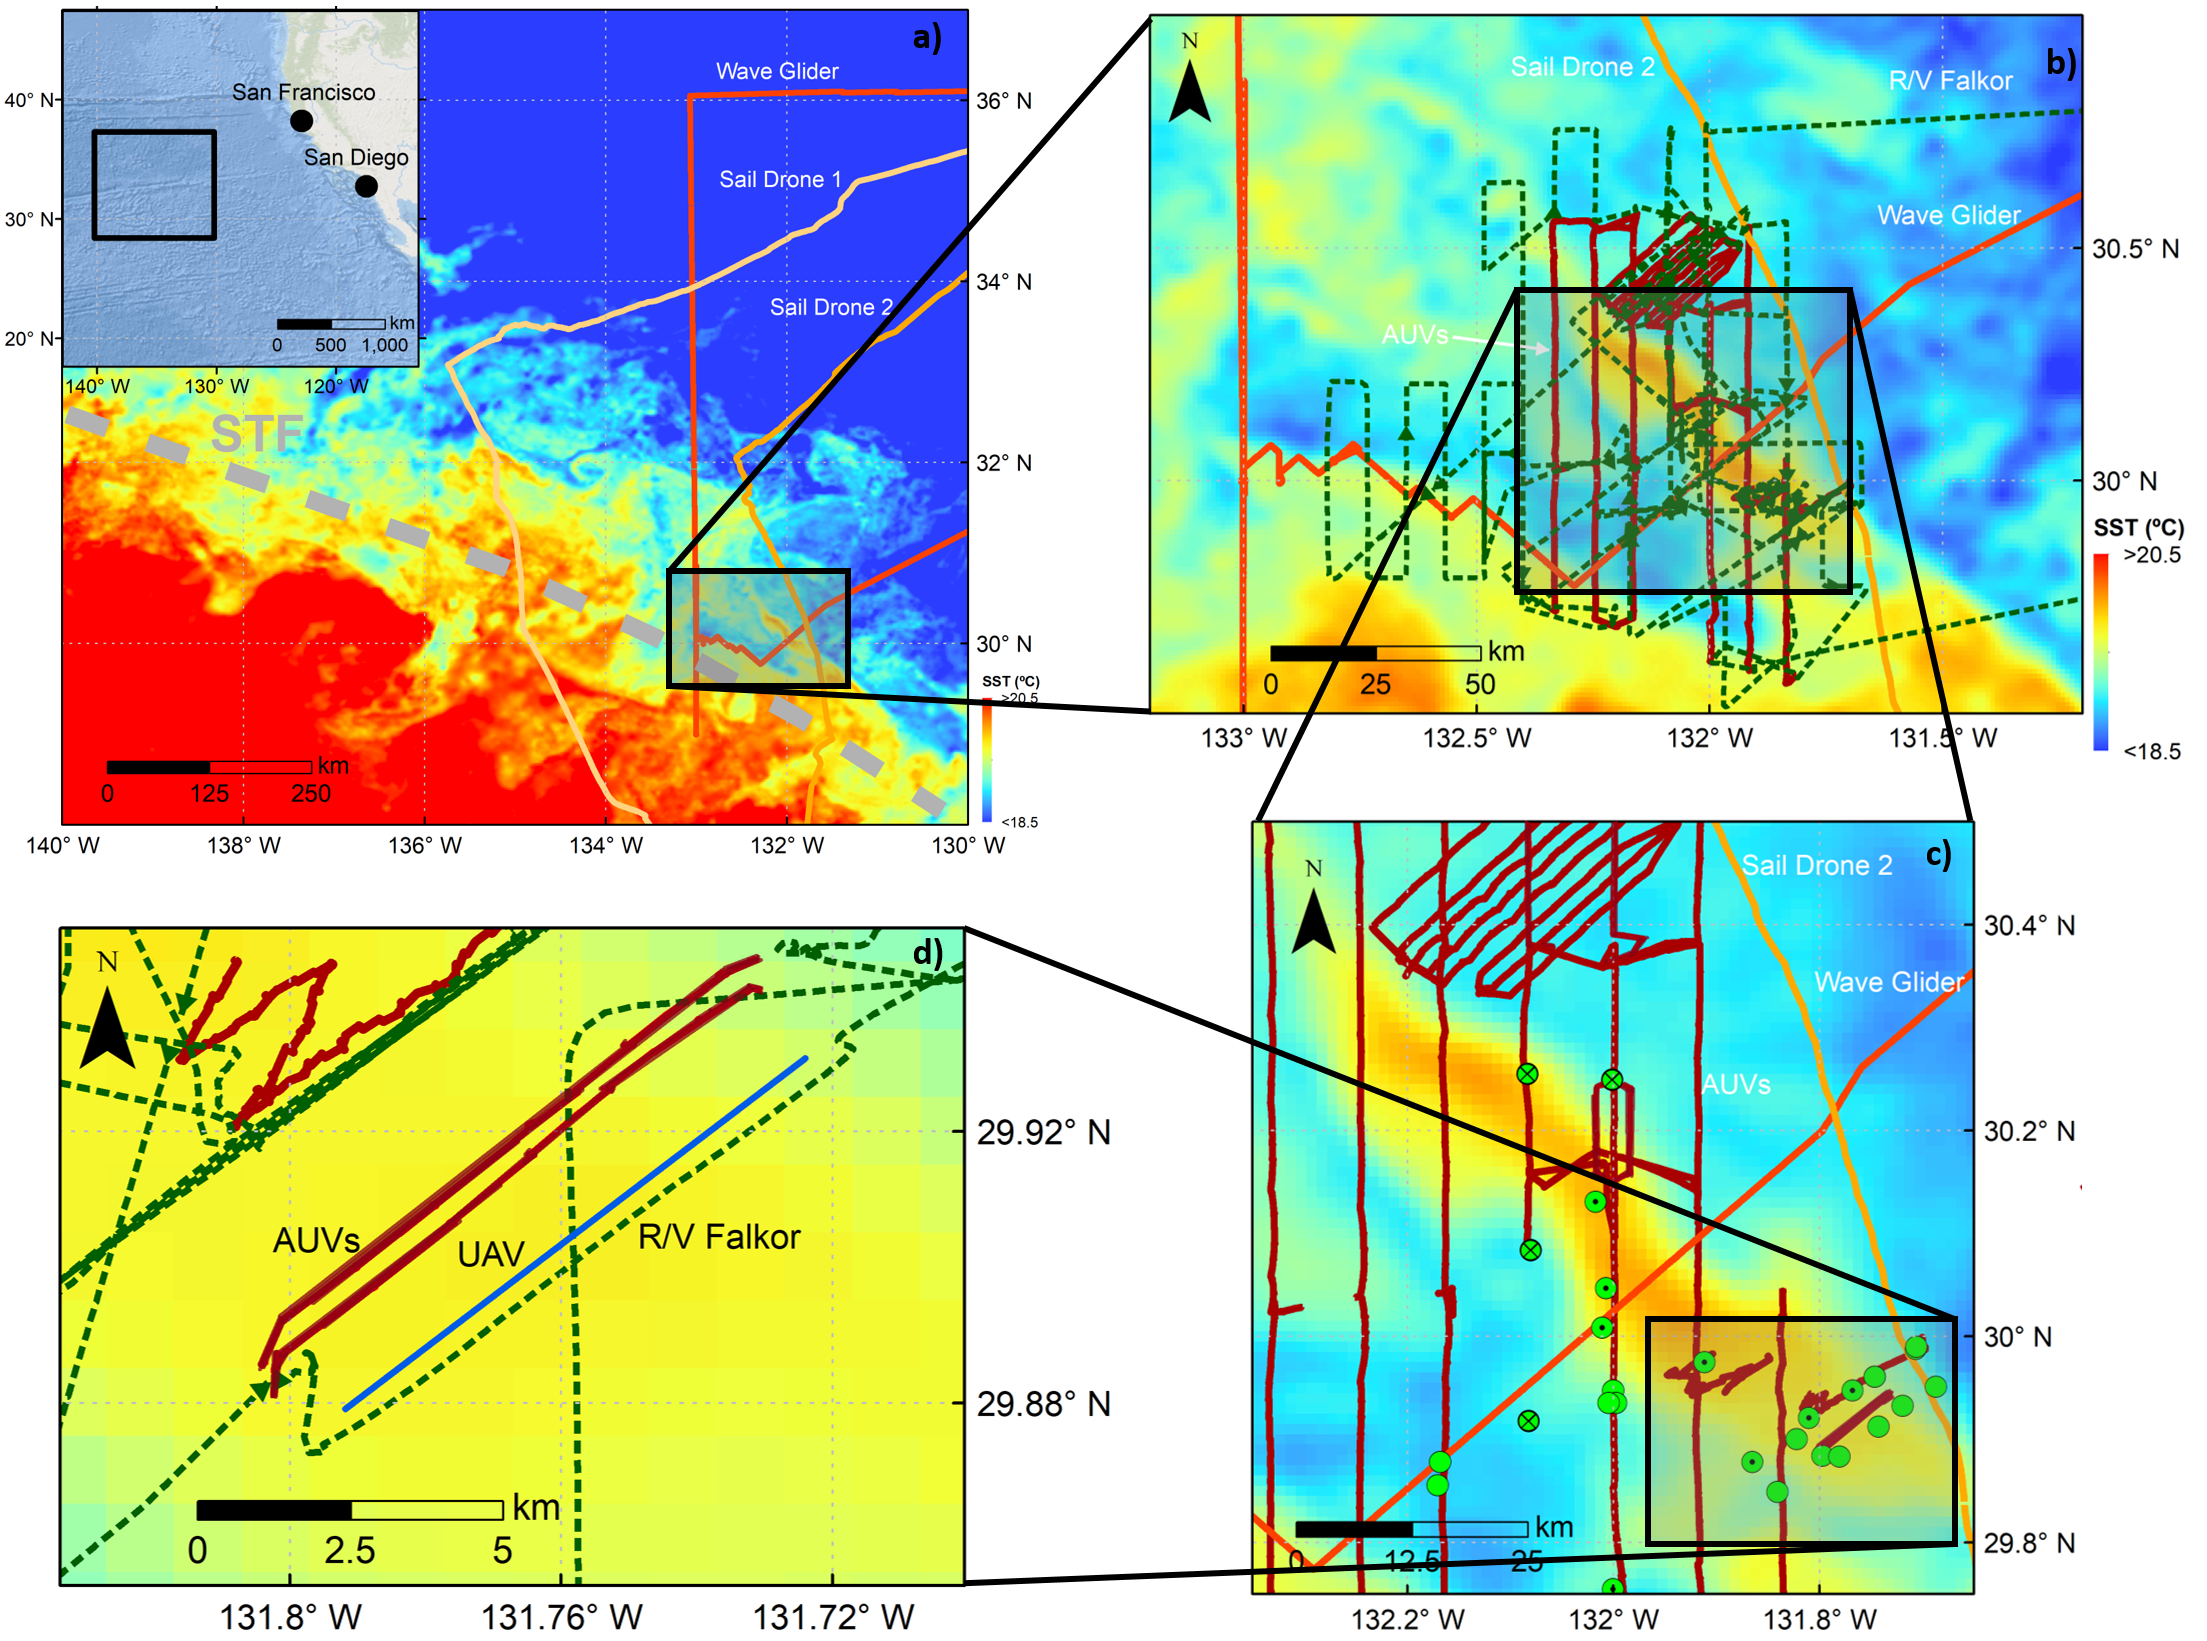
\includegraphics[width=1\linewidth]{figs/fig_multiscale.png}
    \caption{Figure that show the study area and different scales of the target oceanographic feature (Northern Pacific Subtropical Front)- From larger to submesoscale using pre model results (\rpsm{Task to: Renato}}
    \label{fig:block}
\end{figure}

\begin{figure}
    \centering
    \missingfigure[figwidth=0.7\textwidth]{Figure that show the different assets used in our mission highlighting  the coordinate nature of the approach used (\rpsm{Task to: João, José Pinto  LSTS group}}
    \label{fig:block}
\end{figure}

